\subsection{Brugsmønsterrealisering}
I dette afsnit vil der blive lavet en brugsmønsterrealisering, hvor de funktionelle krav som er udtrykt i brugsmænstrene fra afsnit \ref{section: detailed_usemodels} vil blive realiseret.

% -----------------------------------------------------------------------------------------------------------------
\subsubsection{Systemsekvensdiagram}
Et systemsekvensdiagram er et sekvensdiagram der viser systemhændelserne for ét scenarie af et brugsmønster. Diagrammet viser hvordan aktørerne interagerer med systemet for at opfylde brugsmønstret. Diagrammet viser systemet som en ‘black box’, hvilket betyder at man ikke kan se hvad der sker inde i systemet, men kun hvad der sker udenfor systemet. På diagrammet ses det, hvordan aktørerne genererer systembegivenheder og hvad systemets output er. Ydermere viser diagrammet den ‘tidslinje’ begivenhederne sker i. \\

\begin{figure}[ht]
    \centering
    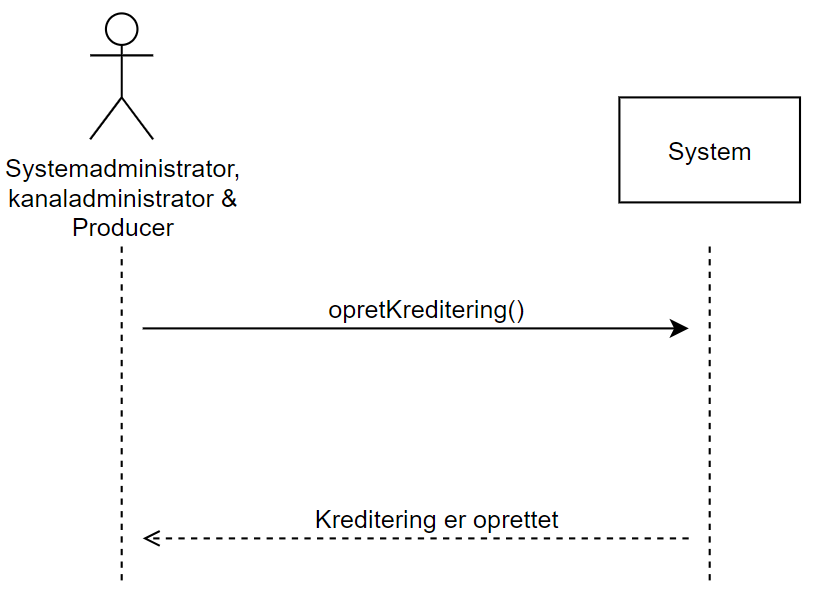
\includegraphics[scale=0.45]{figures/systemsekvensdiagrammer/opretKreditering.PNG}
    \caption{Systemsekvensdiagram for "Opret Kreditering"}
    \label{fig:systemsekvensdiagram_opretKreditering}
\end{figure}

På figur \ref{fig:systemsekvensdiagram_opretKreditering} ser man, at aktøren (Systemadministrator, kanaladministrator eller Producer) kalder metoden opretKreditering ind til systemet, som returnerer at en kreditering er blevet oprettet. Man kan altså ikke se hvordan krediteringen bliver oprettet, og det holdes dermed til hvad der sker uden for systemet. Ud over det ovenstående (system)sekvensdiagram er det valgt at medtage systemsekvensdiagrammer for \textit{godkendKreditering}, \textit{opretProducer}, \textit{sePersonInfo} og \textit{læsKreditering}, som kan findes i bilag \ref{section: systemsekvensdiagrammer}. \\


Efter systemsekvensdiagrammerne er lavet, finder man de operationer systemsekvensdiagrammet kræver. Man kigger altså her ikke længere blot udenfor systemet, men ser på præcis hvordan 'flowet' for brugsmønstret udvikles. Til dette skal man kigge på kontrakter for systemfunktioner.


% -----------------------------------------------------------------------------------------------------------------
\subsubsection{Kontrakter for systemfunktioner}
En systemoperationskontrakt beskriver en operations ansvar, altså hvad en operation har forpligtet sig til. Kontrakten lægger vægt på hvad en operation ændrer på, og ikke på hvordan det ændre sig. En kontrakt kan derfor anses som værende en formel beskrivelse af en operation.\\
Systemoperationskontrakten indeholder navnet på operationen, krydsreferencer til de relevante brugsmønstre, beskrivelse af ansvaret, det output operationen genererer, samt pre- og postkonditioner for operationen. \\


Pre- og postkondinitionerne er stilbilleder af systemet på det givne tidspunkt operationen bliver kaldt. De beskriver altså systemets tilstand før og efter at operationen har kørt. Postkonditioner skal altid noteres i datid, som for eksempel “Købet blev foretaget”, da det er en ting der er sket, og ikke sker.\\


Det er valgt at lave operationskontrakter for de samme operationer som ved systemsekvensdiagrammerne, da disse operationer viser essensen af den logik der skal implementeres. I tabel \ref{tab:kontrakter_opret_kreditering} ses et eksempel på en sådan kontrakt for operationen: \textit{opretKreditering}. De resterende kontrakter kan findes i bilag \ref{section: systemfunktionskontrakter}.


%------------------------ Opret kreditering -------------------------------
\begin{table}[H]
    \begin{tabularx}{\textwidth}{|>{\RaggedRight}p{4cm}|>{\RaggedRight}X|}
        \hline
        \multicolumn{2}{|X|}{\textbf{Opret kreditering}}\\
        \hline
        \textbf{System operation}       & \textbf{opretKreditering} \\ \hline
        \textbf{Krydshenvisning}        & Use case: Opret Kreditering \\ \hline
        \textbf{Ansvar}& At oprette krediteringer og sende den videre til godkendelse hvis prækonditionen er opfyldt, og                                       følgende betingelser er sande: \\
                                        & \\
                                        & \quad 1. Minimumskravene er opfyldt\\
                                        & \quad 2. Alle oplysninger er indtastet korrekt \\
                                        & \\
                                        & Hvis ikke ovenstående er sande, oprettes krediteringen ikke, og brugeren bliver informeret herom \\ \hline
        \textbf{Output}& \quad 1. Produceren får besked om krediteringen er oprettet \\ 
                                        & \quad 2. System- og/eller kanaladministrator får besked om en nyoprettet kreditering \\\hline
        \textbf{Prækonditioner}         & Logget ind som kanal- eller systemadministrator \\ \hline
        \textbf{Postkonditioner}        & En ny kreditering er oprettet i systemet \\ \hline
    \end{tabularx}
    \caption{Systemfunktionskontrakt 'Opret kreditering'}
    \label{tab:kontrakter_opret_kreditering}
\end{table}



% -----------------------------------------------------------------------------------------------------------------
\subsubsection{Operationssekvensdiagram}
Operationssekvensdiagrammet viser systemet som en ”white box”, hvor man kan se hvad der sker inde i systemet. Sekvensdiagrammet bruges til at identificere systemfunktioner, da de begivenheder der vises i diagrammet er de funktioner systemet skal indeholde. Et eksempel på et operationssekvensdiagram for "Læs Kreditering" kan ses på figur \ref{fig:op_read_credit}.

\begin{figure}[H] % <--- HUSK AT ÆNDRE MIG :-)
\centering
\includegraphics[scale=0.9]{figures/Operationssekvensdiagrammer/læsKreditering.pdf}
\caption{Operationssekvensdiagram: Læs kreditering}
\label{fig:op_read_credit}
\end{figure}


På figur \ref{fig:op_read_credit} ses det, hvad der finder sted i systemet når brugeren vil læse en kreditering. Brugeren starter ud med at kalde en metode i desktop-klienten, der kalder en \texttt{GET} metode i REST api'et, hvor id'et eller navnet på en produktion er med som parameter. Api'et udfører derefter SQL-forespørgelse i databasen, for at hente den specifikke kreditering. Databasen sender et resultatsæt tilbage, og api'et sender en HTTP kode sammen med et JSON object til desktop-klienten. JSON objektet er den produktion brugeren gerne vil læse krediteringerne til. Desktop-klienten håndterer derefter JSON objektet, så det pænt vises til brugeren. De resterende operationssekvensdiagrammer kan findes i bilag \ref{section: operationssekvensdiagrammer}.





